\documentclass[11pt,border=6pt]{standalone}
\usepackage{fontspec}
\usepackage{tikz}
\begin{document}
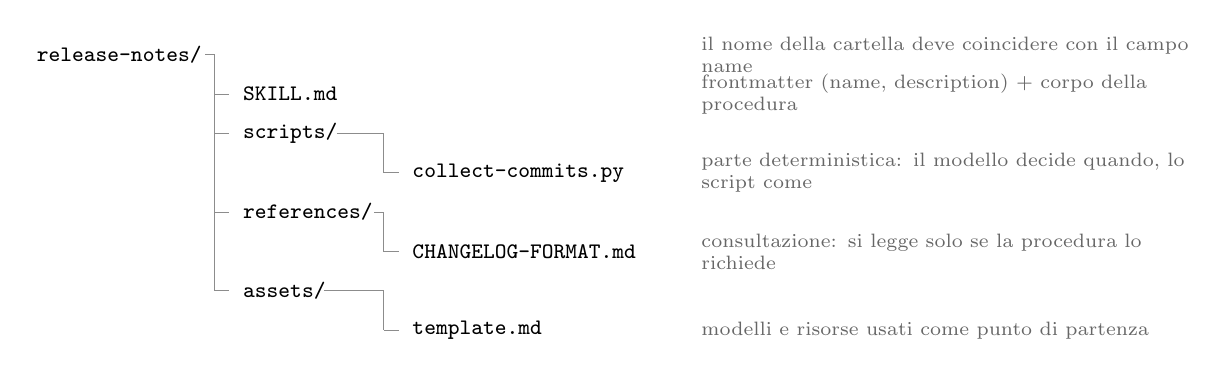
\begin{tikzpicture}
% anatomia di una skill: cartella, file obbligatorio, cartelle opzionali

% righe: nome in monospazio, annotazione a destra
\node[anchor=west, font=\ttfamily\footnotesize] (n0) at (0.00,0.00) {release-notes/};
\node[anchor=west, font=\scriptsize, text=black!60, text width=6.2cm, align=left] at (8.44,0.00) {il nome della cartella deve coincidere con il campo name};
\node[anchor=west, font=\ttfamily\footnotesize] (n1) at (2.62,-0.50) {SKILL.md};
\node[anchor=west, font=\scriptsize, text=black!60, text width=6.2cm, align=left] at (8.44,-0.50) {frontmatter (name, description) + corpo della procedura};
\node[anchor=west, font=\ttfamily\footnotesize] (n2) at (2.62,-1.00) {scripts/};
\node[anchor=west, font=\ttfamily\footnotesize] (n3) at (4.77,-1.50) {collect-commits.py};
\node[anchor=west, font=\scriptsize, text=black!60, text width=6.2cm, align=left] at (8.44,-1.50) {parte deterministica: il modello decide quando, lo script come};
\node[anchor=west, font=\ttfamily\footnotesize] (n4) at (2.62,-2.00) {references/};
\node[anchor=west, font=\ttfamily\footnotesize] (n5) at (4.77,-2.50) {CHANGELOG-FORMAT.md};
\node[anchor=west, font=\scriptsize, text=black!60, text width=6.2cm, align=left] at (8.44,-2.50) {consultazione: si legge solo se la procedura lo richiede};
\node[anchor=west, font=\ttfamily\footnotesize] (n6) at (2.62,-3.00) {assets/};
\node[anchor=west, font=\ttfamily\footnotesize] (n7) at (4.77,-3.50) {template.md};
\node[anchor=west, font=\scriptsize, text=black!60, text width=6.2cm, align=left] at (8.44,-3.50) {modelli e risorse usati come punto di partenza};

% connettori ad albero
\draw[black!45] (2.26,0.00) -- (2.38,0.00);
\draw[black!45] (2.38,0.00) -- (2.38,-3.00);
\draw[black!45] (2.38,-0.50) -- (2.57,-0.50);
\draw[black!45] (2.38,-1.00) -- (2.57,-1.00);
\draw[black!45] (2.38,-2.00) -- (2.57,-2.00);
\draw[black!45] (2.38,-3.00) -- (2.57,-3.00);
\draw[black!45] (3.93,-1.00) -- (4.53,-1.00);
\draw[black!45] (4.53,-1.00) -- (4.53,-1.50);
\draw[black!45] (4.53,-1.50) -- (4.72,-1.50);
\draw[black!45] (4.41,-2.00) -- (4.53,-2.00);
\draw[black!45] (4.53,-2.00) -- (4.53,-2.50);
\draw[black!45] (4.53,-2.50) -- (4.72,-2.50);
\draw[black!45] (3.77,-3.00) -- (4.53,-3.00);
\draw[black!45] (4.53,-3.00) -- (4.53,-3.50);
\draw[black!45] (4.53,-3.50) -- (4.72,-3.50);
\end{tikzpicture}
\end{document}
